\chapter{大規模な問題におけるペトリネット変換}
\label{main_survey}

\section{効率よく解を探索するためのマシンリソース配置}
量子アニーリングは,変数の数が少ない場合により効率的に最適解を探索できる特性がある.この特性,問題の解探索に必要な量子ビットの数が変数の数に依存するためである.変数が少ないほど解の探索空間が小さくなり最適解に到達しやすくなる.このため,量子アニーリングを用いる場合は,対象問題を可能な限りコンパクトに表現し変数の数を削減することが重要である.特に,大規模問題を効率的に解くためには,ペトリネット変換や問題分割などの手法を用いて問題のサイズを適切に縮小することが必要である.

\begin{figure}[H]
    \centering
    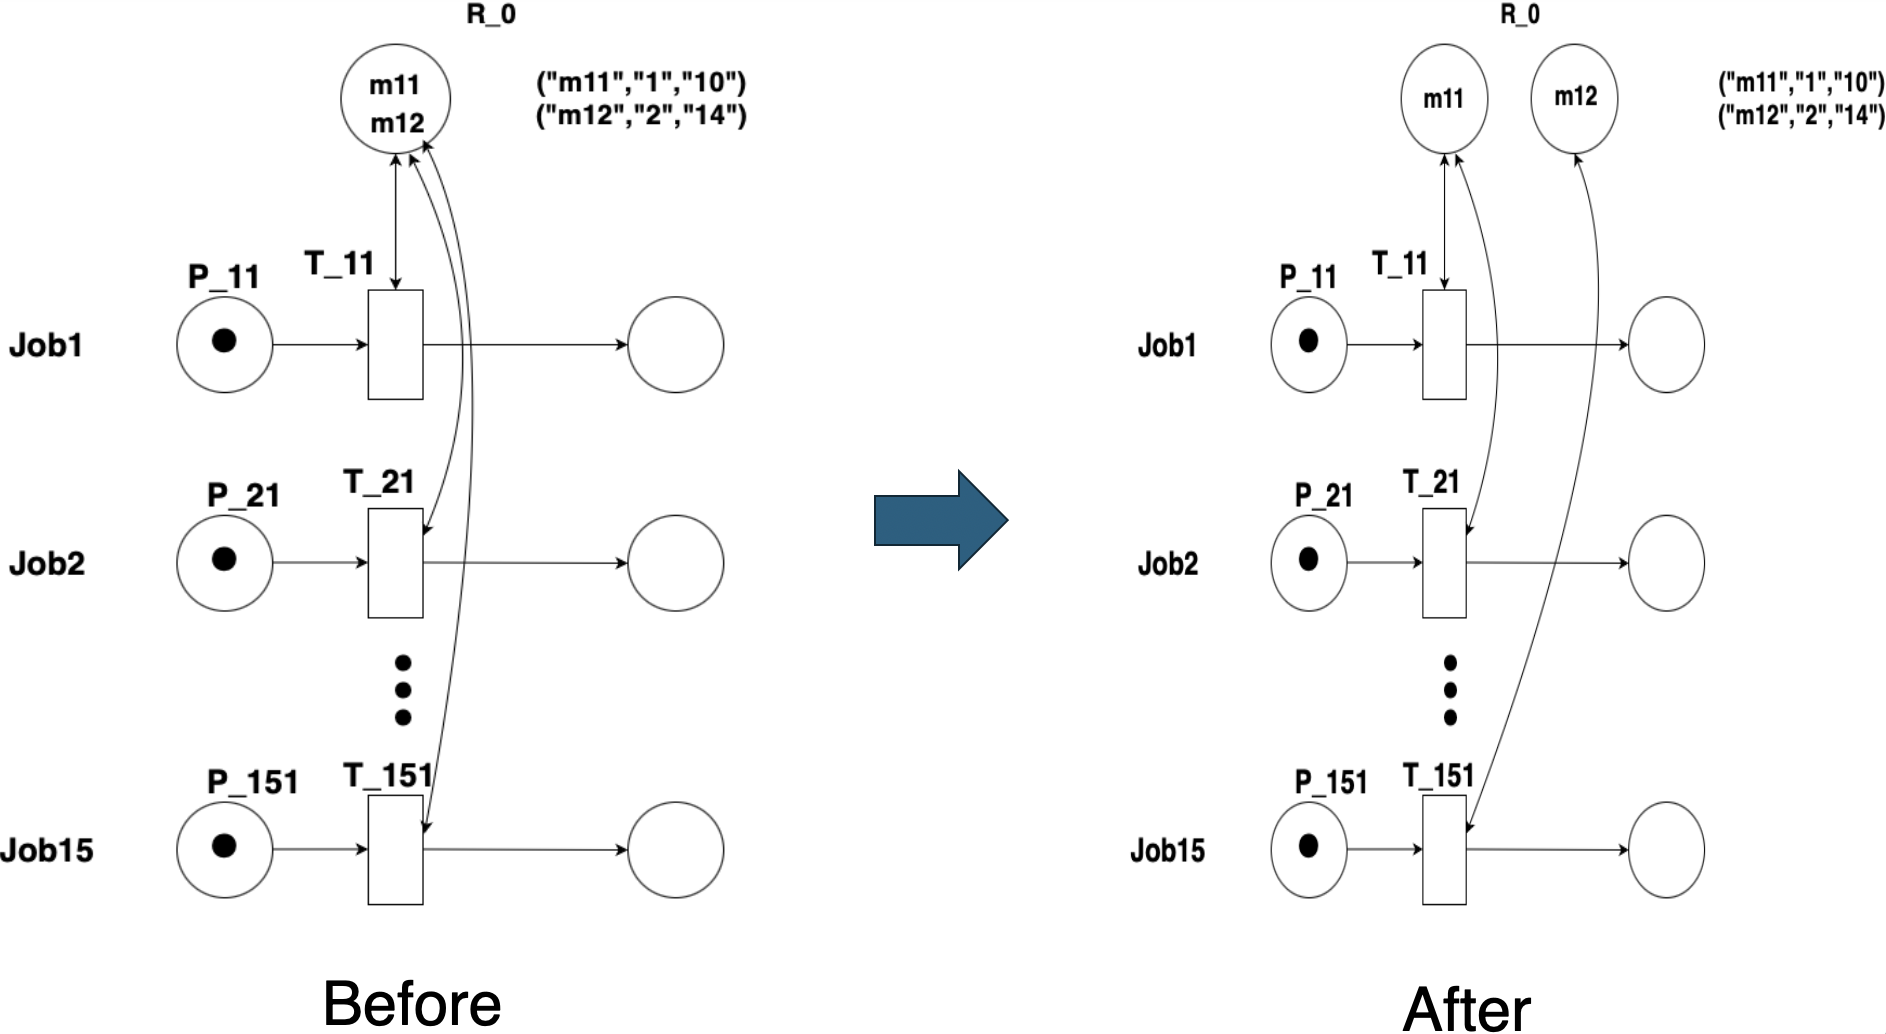
\includegraphics[width=0.8\linewidth, height=8cm]{./images/transformation.png}
    \caption{変数削減のためのペトリネット変換}
    \label{fig:fig2}
\end{figure}

図\ref{fig:fig2}は対象問題のペトリネットモデルを変換した図になる.このモデル変換は以下の二段階のプロセスで構成される.

\begin{enumerate} 
\item リソースの事前割り当てを適用することによりペトリネットモデルを変換する.ペトリネットモデルを変換するためのエネルギー関数が(\ref{eqn:tran})式である.
\begin{align} 
min \sum_{m \ne m_i}^M \left( \sum_t^T a_{m_i,t} \cdot x_{m_i,t} - \sum_t^T a_{m,t} \cdot x_{m,t}\right)^2 + \left(1 - \sum_t^T x_{m,t} \right)^2 \label{eqn:tran} 
\end{align}

\item (\ref{eqn:tran})式を処理時間またはリソースコストを最適化を行うことで効率的なリソース配置をする.
\end{enumerate}

変数の数は$r \times k \times t$(ここで,$r$はマシンリソース数,$k$は制限の最大時刻,$t$はタスク数)で表される.だが,ペトリネットモデルの変換を行うことにより変数の数が$k \times t$に削減される.この削減により,最適化計算の規模が縮小し計算効率が向上する.

\section{評価実験}

比較とかする




